\documentclass[10pt, a4paper]{article}

\usepackage[left=0.6in, right=0.6in, top=0.5in, bottom=0.5in]{geometry}
\usepackage{enumitem}
\usepackage{hyperref}
\usepackage{titlesec}
\usepackage{graphicx}
\usepackage{fontawesome}
\usepackage{tikz}
\usepackage{xcolor}
\usepackage{tabularx}
\usepackage{array}
\usepackage{colortbl}
\usepackage[sfdefault]{inter}
\usepackage[T1]{fontenc}
\usepackage{parskip}
\usepackage{multicol}

% Colors
\definecolor{accent}{RGB}{41, 98, 155}
\definecolor{darkgray}{RGB}{50, 50, 50}
\definecolor{lightgray}{RGB}{100, 100, 100}
\definecolor{verylightgray}{RGB}{245, 245, 245}
\definecolor{tablegray}{RGB}{230, 230, 230}

\hypersetup{colorlinks=true, linkcolor=accent, urlcolor=accent}

% Section styling
\titleformat{\section}{\large\bfseries\color{accent}}{}{0em}{}[\vspace{-0.3em}\textcolor{accent}{\rule{\linewidth}{1pt}}]
\titlespacing{\section}{0pt}{0.8em}{0.4em}

\titleformat{\subsection}{\normalsize\bfseries\color{darkgray}}{}{0em}{}
\titlespacing{\subsection}{0pt}{0.6em}{0.2em}

\pagestyle{empty}
\setlength{\parindent}{0pt}

\newcolumntype{L}[1]{>{\raggedright\arraybackslash}p{#1}}
\newcolumntype{R}[1]{>{\raggedleft\arraybackslash}p{#1}}

\begin{document}

% Header
\begin{minipage}[t]{0.62\textwidth}
\vspace{0pt}
{\small\color{lightgray}CONSULTANT PROFILE}

\vspace{0.3em}
{\LARGE\bfseries\color{darkgray} Frej Sundqvist}

\vspace{0.8em}
{\small
Fullstack developer with experience building web applications from scratch to production. Strong background in computational physics. Specializes in modern web technologies. Thrives in collaborative environments with hands-on technical involvement.
}

\vspace{0.8em}
{\small
{\color{accent}\faEnvelopeO} frejsundqvist@protonmail.com
}
\end{minipage}%
\hfill
\begin{minipage}[t]{0.35\textwidth}
\vspace{0pt}
\raggedleft
\begin{tikzpicture}
    \clip (0,0) circle (1.5cm);
    \node at (0.1, -0.4) {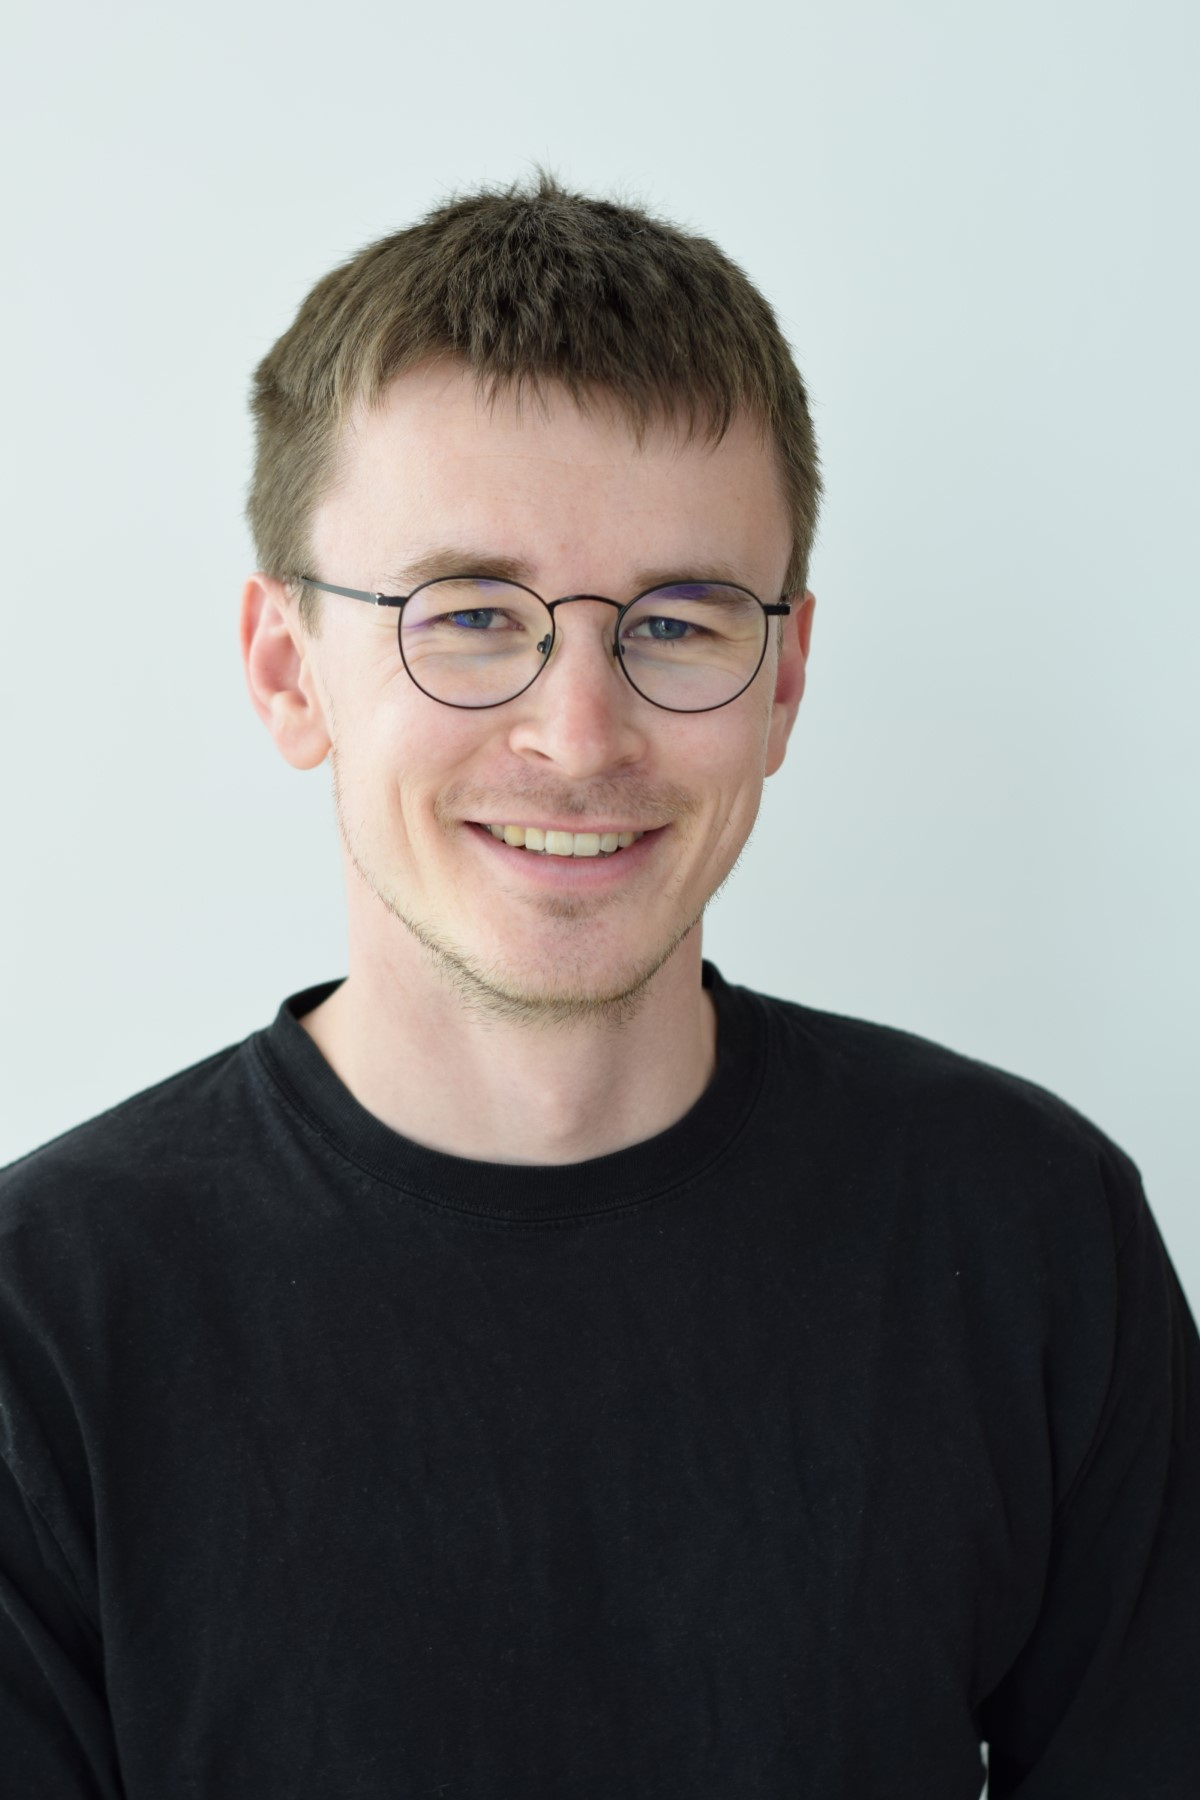
\includegraphics[height=4.5cm]{./assets/profile_pic_small.jpg}};
\end{tikzpicture}

\vspace{0.5em}
\raggedright
{\small\bfseries\color{accent}CURRENT ROLES}\\
{\small System Developer\\UI/UX Team Lead}

\vspace{0.5em}
{\small\bfseries\color{accent}CORE SKILLS}\\
{\small Svelte/SvelteKit\\Python/Django}

\vspace{0.5em}
{\small\bfseries\color{accent}LANGUAGES}\\
{\small Swedish (Native)\\English (Fluent)\\German (Fluent)\\Norwegian (Fluent)}

\vspace{0.5em}
{\small\bfseries\color{accent}INDUSTRIES}\\
{\small Satellite/Space Tech\\Fisheries\\Tourism\\Infrastructure\\Consulting}
\end{minipage}

\vspace{0.5em}
\noindent\rule{\linewidth}{0.5pt}

% Two column layout for Work Experience and Education
\begin{minipage}[t]{0.48\textwidth}
\section*{Work Experience}
{\small
\begin{tabular}{@{}L{2.2cm}L{5cm}@{}}
2024 -- present & System Developer / KSAT \\
2021 -- 2024 & Fullstack Engineer, Tech Lead / Capia AS \\
\end{tabular}
}
\end{minipage}%
\hfill
\begin{minipage}[t]{0.48\textwidth}
\section*{Education}
{\small
\begin{tabular}{@{}L{2.2cm}L{5cm}@{}}
2015 -- 2021 & M.Sc. Engineering Physics / Ume\aa\ University \\
2018 -- 2019 & Exchange year / JMU W\"urzburg, Germany \\
\end{tabular}
}
\end{minipage}

\section*{Tools, Technologies \& Methods}
{\small
\begin{tabularx}{\textwidth}{@{}L{3.2cm}X@{}}
\rowcolor{verylightgray}
\textbf{Languages} & Python, Java, TypeScript, JavaScript, C, Rust, SQL, Bash \\
\textbf{Frontend} & Svelte, SvelteKit, React, Next.js, Tailwind CSS, HTML, CSS, LESS, Webpack, Vite \\
\rowcolor{verylightgray}
\textbf{Backend} & Django, Django REST Framework, FastAPI, Quarkus, Flask, REST APIs, GraphQL, Celery \\
\textbf{Databases} & PostgreSQL, MySQL, PostGIS, Redis, Flyway \\
\rowcolor{verylightgray}
\textbf{DevOps} & Docker, Kubernetes, GitHub Actions, Bitbucket Pipelines, Nginx, OpenTelemetry, Prometheus, Grafana \\
\textbf{Azure} & Entra ID, Blob Storage, Key Vault, Application Insights, Service Bus, Container Apps, Azure OpenAI \\
\rowcolor{verylightgray}
\textbf{Workflow} & Apache Airflow, Kafka, Temporal, Dagster \\
\textbf{ML/AI} & PyTorch, LLMs, Neural Networks, Image Segmentation, Pandas, NumPy \\
\rowcolor{verylightgray}
\textbf{Auth/IAM} & Keycloak, OpenFGA, OpenID Connect, OAuth 2.0, JWT \\
\textbf{Other} & Git, Linux, Google Cloud, Cloudflare, Agile, Scrum \\
\end{tabularx}
}

\section*{Project Experience}

\subsection*{KSAT -- LLM Integration in Web Applications}
{\small\color{lightgray}2025 -- present}

{\small
\textbf{Project:} Integration of Large Language Models into customer web application to enhance user productivity and automate workflows.

\textbf{Role:} System Developer, UI Lead Developer

\begin{itemize}[noitemsep, leftmargin=1.2em, topsep=0.2em]
    \item Designing and implementing LLM-powered features in production applications
    \item Building prompt engineering pipelines and evaluation frameworks
    \item Integrating with Azure OpenAI services
\end{itemize}

\textbf{Technologies:} Python, Azure OpenAI, Svelte, SvelteKit, TypeScript, Tailwind CSS
}

\vspace{0.8em}
\subsection*{KSAT -- Central Authorization Service}
{\small\color{lightgray}2025 -- present}

{\small
\textbf{Project:} Development of centralized authorization service for cross-team use across the organization.

\textbf{Role:} System Developer

\begin{itemize}[noitemsep, leftmargin=1.2em, topsep=0.2em]
    \item Designing authorization models using OpenFGA
    \item Cross-team collaboration on authorization requirements
    \item Integration with existing services and applications
\end{itemize}

\textbf{Technologies:} OpenFGA, Python, Java, Quarkus
}

\vspace{0.8em}
\subsection*{KSAT -- Customer Portal Development}
{\small\color{lightgray}2024 -- present}

{\small
\textbf{Project:} End-to-end design and development of customer portal. Cloud-hosted fullstack application.

\textbf{Role:} Fullstack Developer, UI Lead Developer, Database Designer

\begin{itemize}[noitemsep, leftmargin=1.2em, topsep=0.2em]
    \item Designing and building portal from scratch to production
    \item Database design and API architecture
    \item Frontend development with Svelte/SvelteKit
    \item Cloud deployment and infrastructure
\end{itemize}

\textbf{Technologies:} Svelte, SvelteKit, TypeScript, Tailwind CSS, Python, Java, Quarkus, PostgreSQL, Docker, Azure Container Apps, OpenTelemetry, Temporal, OpenFGA
}

\vspace{0.8em}
\subsection*{Capia AS -- Live Fish Administration System}
{\small\color{lightgray}2022 -- 2024}

{\small
\textbf{Project:} Full lifecycle development of administration system for live fish management in the aquaculture industry. Built from scratch to production deployment.

\textbf{Role:} Tech Lead, Lead Developer

\begin{itemize}[noitemsep, leftmargin=1.2em, topsep=0.2em]
    \item Led development team and established technical direction
    \item Built complete fullstack application from scratch to deployment
    \item Integrated Keycloak for authentication and authorization
    \item CI/CD pipeline setup and Linux server administration
\end{itemize}

\textbf{Technologies:} Django, React, TypeScript, Tailwind CSS, PostgreSQL, Keycloak, Celery, Nginx
}

\vspace{0.8em}
\subsection*{Capia AS -- Road Infrastructure Analytics Platform}
{\small\color{lightgray}2021 -- 2022}

{\small
\textbf{Project:} Development of analytics platform for road maintenance insights and infrastructure condition monitoring.

\textbf{Role:} Fullstack Developer

\begin{itemize}[noitemsep, leftmargin=1.2em, topsep=0.2em]
    \item Built web application for road condition data visualization
    \item Implemented geospatial data processing with PostGIS
    \item Developed APIs for infrastructure monitoring data
\end{itemize}

\textbf{Technologies:} Django, React, Python, PostgreSQL, PostGIS, Docker, Nginx, Celery, Tailwind CSS, Apache Airflow
}

\vspace{0.8em}
\subsection*{Capia AS -- Tourism Industry Analytics Platform}
{\small\color{lightgray}2021 -- 2022}

{\small
\textbf{Project:} Development of register and analytics platform for the tourism industry in Tromsø, built for local authorities.

\textbf{Role:} Fullstack Developer, Project Lead, Customer Contact

\begin{itemize}[noitemsep, leftmargin=1.2em, topsep=0.2em]
    \item Built web application for tourism data registration and analytics
    \item Direct customer interaction and requirements gathering
    \item Implemented data visualization and reporting features
\end{itemize}

\textbf{Technologies:} Django, React, Python, PostgreSQL, PostGIS, Docker, Nginx, Celery, Tailwind CSS
}

\vspace{0.8em}
\subsection*{Capia AS -- Smart Car Fleet Insights Hub}
{\small\color{lightgray}2021 -- 2022}

{\small
\textbf{Project:} Consulting project developing insights platform for smart car fleet management with third-party API integrations and data visualization.

\textbf{Role:} Consultant, Developer

\begin{itemize}[noitemsep, leftmargin=1.2em, topsep=0.2em]
    \item Integrated external vehicle APIs for fleet data collection
    \item Built data visualization dashboards for fleet insights
    \item Developed data processing pipelines
\end{itemize}

\textbf{Technologies:} FastAPI, Python, Pandas, NumPy, PostgreSQL, Redis, REST APIs
}

\end{document}
